\chapter{Design and Implementation}
\lstset{language=Java}
This section includes both design decisions and implementation details.

One of the basic implementation choices was the programming language used to implement the software.
Several properties had to be considered.
The framework is intended for use by researchers, if it is implemented in a language that is not widely used the adoption of the framework will be affected.
Tool support was also a significant consideration.
The availablity of tools such as development environments, debuggers and profilers can vastly improve the quality of software.
With a motivation of the project being to reduce bespoke research software, the libraries that are available must be considered

After consideration of all three factors outlined Java was selected as the programming language for the implementation.
Java has good tool support, a high number of available libraries and is used sufficiently in the research community.
An additional benefit of Java is that requirement Req:POR is made considerably simpler by the Java virtual machine.

\section{Framework}
In this section I will outline the design decisions that directly effect the framework produced and how it was implemented.

\subsection{Complex Numbers}
Complex numbers are central to Quantum Computing.
As such, any attempt to simulate the behaviour of a Quantum Circuit must handle complex numbers.

There are really only two ways to handle the existence of complex numbers.
One can represent a complex number explicitly as a pair of floating point numbers, or to encapsulate the representation inside a ``complex number'' data structure.

The framework uses the second of these options and provides the ``Complex'' class.
This was chosen for several reasons.
The primary reason was to reduce the risk of programming errors effecting the simulation.
If complex multiplication, addition and other operations had to be replicated throughout the framework code base, and the code base of any research work, the likelihood of implementation error is much higher, and the tests required to find the error become more specific.
It is much better software engineering practice to encapsulate the properties, real and imaginary values, and the operations on those properties, arithmetic etc.

A season reason is that after brief research online, there are complex number libraries already available.
This reuse of previously written software can also reduce the likelihood of errors in the code.
This is not necessarily due to the software being written by people that are more intelligent or that are better programmers, or even that the software has been explicitly tested more thoroughly than if I were to write a complex number class.
It is due to the size of the deployment footprint.
The number of times the software has previously been deployed, and therefore the number of times it has been implicitly tested by users.

The third reason is that one of the principles behind producing the framework is the attempt to try standardise the research from different researchers.
Without the provision of this ``Complex'' class one researcher could use Cartesian representation, two floating point values, while a second researcher could use the Polar representation, also two floating point values.
If the documentation of the software produced by the two researchers did not mention the representation used, a third researcher could try combine, or compare, the two pieces of software using the framework.
The third researcher is likely to receive very confusing and highly misleading results.
The provision of a Complex class that is used throughout the framework where complex numbers need to be used will reduce the risk of such an event.

The implementation of the Complex class is based on an implementation provided as part of a ``Complex Function Grapher''\cite{compimp}.
The Complex class provides both Cartesian form $real + imaginary$, through \lstinline{real()} and \lstinline{imag()} returning the real and imaginary components respectively, and Polar form $re^{i\theta}$, through \lstinline{mod()} and \lstinline{arg()} returning $r$ and $\theta$ respectively.
The implementation has been adapted to better suit this application.
A calculation of the euclidean distance between two complex numbers is provided.
A second addition is the ability to \lstinline{parseComplex} in a similar way to \lstinline{parseInt} or \lstinline{parseDouble} provided by the standard Integer and Double classes respectively.
This allows a string such as ``$2+3i$'' to be input by a user and for a Complex object to be created with a real component of $2$ and imaginary component of $3$.

\subsection{Matrices}
As seen in Equation \ref{eq:notexplanded} the application of a quantum gate is simply the application of a unitary operation, represented as a matrix, to a quantum state.
The framework has to implement matrices in some way.

There are several possible representations.
The framework could either use an explicit representation, two-dimensional arrays, or could provide a Matrix data structure.

The framework has been designed to use the data structure encapsulation as the matrix representation.
The justification is identical to that discussed above.
Matrix operations are easy to get wrong in implementation and there are matrix libraries for many languages.
The incomplete documentation argument also holds with matrices.
If the framework were to just simply represent matrices as two dimensional arrays, two researchers could order the dimensions differently leading to similar problems to that of conflicting complex representations for the third researcher.

\lstset{language = XML,
basicstyle=\footnotesize,
breakatwhitespace=false,
numbers=none,
breaklines=true}
\begin{figure}
\begin{center}
\subfigure[XML Definition]{
\lstinputlisting{pauliixml.tex}
\label{pauliixmllisting}
}
\hspace{20pt}
\subfigure[Matrix]{$
\begin{pmatrix}
1 && 0 \\
0 && 1
\end{pmatrix}$}
\end{center}
\caption{Pauli-I Gate}
\label{code:pauliixmldef}
\end{figure}

The implementation of the Matrix used in the application is based on the JAMA Matrix package\cite{javamatrix}.
The JAMA Matrix package provides matrices of double values.
For use in the framework this needed to be updated so that it provides matrices of Complex objects and performs all the required operations as though they are matrices of complex numbers.

The JAMA Matrix package provides extra functionality for matrices of doubles that are not required for the framework.
In the conversion from double matrices to Complex matrices this additional functionality was removed.

The JAMA Matrix package does not include the tensor product operation.
This operation is used heavily when applying single qubit gates to multi-qubit systems and so was specifically developed.

As is explained in Section \ref{sec:testsuitestruc} custom unitary matrices are needed and used as part of the test cases.
This requires these unitary matrices to be stored in a form that can be distributed between researchers.
As with all elements of this framework that needs to be distributable, XML is used to store these matrices.
The XML structure and defined matrix can be seen in Figure \ref{code:pauliixmldef}.
The use of XML was used rather than the Java Serializable interface to ensure that 3rd party applications can be used to modify the stored matrices if required.

\subsection{State}
Quantum states are naturally represented as $2^n\times1$ matrices, vectors.
All unitary operators are implemented simply as the application of $2^n\times2^n$ matrices to these quantum state vectors.

\subsection{Test Suite Structures}
\label{sec:testsuitestruc}
With most heuristic search problems there are a series of test points that are used to measure the suitability of any proffered solution.

For Quantum Algorithms the expected results are the state vectors produced by circuits constructed by the algorithm.
As such it was chosen that a test case would be represented as a pair of state vectors, the stating state and the expected state.
The application of a quantum gate is a simple mapping from a starting state to a resulting state.
When a circuit can be defined as a single unitary operation, a custom quantum gate, this representation seems a natural choice.

For some problems, such as the Deutsch and Deutsch-Jozsa problems, the starting and final state are not information but pure data, they have no context.
As is shown in Section \ref{sec:quantumgates} there is no gate $f$ as is used in the Deutsch and Deutsch-Jozsa algorithms.
This may initially seem a rather strange omission.
However, the $f$ in the Deutsch and Deutsch-Jozsa algorithms are not fixed gates, they are arbitrary unitary operations that are guaranteed to be either constant or balanced.
Therefore it is not sufficient for the test cases to be just the starting and final state but must provide a way for custom unitary matrices to be specified.
With these custom matrices specified, the starting and final states in the test cases for the Deutsch and Deutsch-Jozsa problems are given context and therefore are transformed into meaningful information.

Each circuit produced by quantum algorithm has $n$ qubits.
This means that it can only be evaluated using test cases for $n$ qubits.
Test cases for any other number of qubits would not produce useful results, and are potentially incomputatable due to incorrect matrix dimensions for multiplication.
The notion of a test set was introduced to hold all test cases for a specific $n$.
A search might well find a circuit suited to a specific $n$ with no clear generalisation possible.
All test cases are held within a test set.

However, the power of a quantum algorithm over a quantum circuit is the generality of the algorithm for any $n$.
This means that a single test set is not suitable as it would only evaluate the algorithm for test cases for a single $n$.
The notion of a test suite is introduced.
A test suite is used to hold all the test sets produced for the same problem.
There is only one test set for each distinct value of $n$.
The implemented structure can be seen in Figure \ref{fig:testsuiteclassdiag}.

The number of custom gates that are available to use are constant for all the test cases in the test suite.
This number cannot vary as the algorithms produced must be able to contain only the gates available.
If each test case were able to have a different number of custom gates an algorithm produced could contain the instruction to include ``Custom Gate 4'' but a test case could only provide two custom gates.

The test suite is fully defined in a single XML file.
The XML in Figure \ref{code:paulixtestset} is a sample of such a file.
It is easy to see file structure reflects the internal structure of test suites just described.

\lstset{language = XML,
basicstyle=\footnotesize,
breakatwhitespace=false,
numbers=none,
breaklines=true}
\begin{figure}
\centering
\subfigure[Partial Test Set for Pauli X Gate]{
\label{code:paulixtestset}
\begin{minipage}[c]{%
	   0.4\textwidth}
	   \centering%
% 	   \includegraphics[width=0.8\textwidth]{box}
	   \lstinputlisting{paulixtestcasexml.tex}
\end{minipage}
}
\hspace{5em}
\subfigure[Test Suite Class Diagram]{
\label{fig:testsuiteclassdiag}
\begin{minipage}[c]{%
	   0.4\textwidth}
	  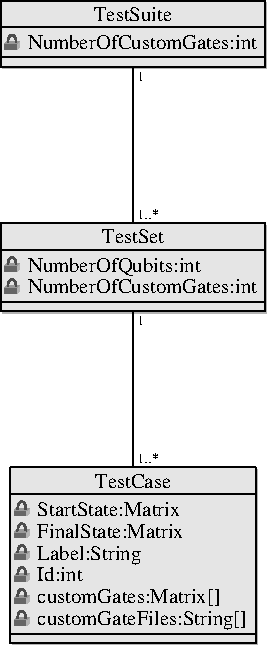
\includegraphics[height=0.4\textheight]{testsuitefig.pdf}
\end{minipage}
% \begin{emp}[classdiag](20, 20)
%   Class.A("TestCase")("-StartState:Matrix","-FinalState:Matrix","-Label:String","-Id:int","-customGates:Matrix[]","-customGateFiles:String[]")();
%   Class.B("TestSet")("-NumberOfQubits:int","-NumberOfCustomGates:int")();
%   Class.C("TestSuite")("-NumberOfCustomGates:int")();
%   % Class.D("SuperPositionalTestSet")()();
%   topToBottom(75)(C, B, A);
%   % D.n = B.s - (0, 50);
%   drawObjects(C, B, A);
%   clink(association)(C, B);
%   item(iAssoc)("1")(obj.nw = C.e);
%   item(iAssoc)("1..*")(obj.ne = B.w);
%   clink(association)(B, A);
%   item(iAssoc)("1")(obj.nw = B.e);
%   item(iAssoc)("1..*")(obj.ne = A.w);
%   % link(inheritance)(D.n -- B.s)
% \end{emp}
}
\caption{Test Suite Structures}
\end{figure}

Separate files are used to encapsulate the test suite specifications rather than including these in the Search Problem Manager configuration file, discussed in Section \ref{sec:manclasses}.
This separation follows the software engineering principle of modularity to ensure that the files remain readable and maintainable.
The framework is intended to improve the ability of researchers to reuse development or other researchers, the creation of test suite specifications can be seen as development.
With this modularity the distribution and reuse of test suite specifications will be much simpler than if the test suite specifications were embedded in the Search Problem Manager configuration file, discussed in Section \ref{sec:manclasses}.

% \begin{figure}
% \centering
% % \begin{emp}[classdiag](20, 20)
% % Class.A("TestCase")("-StartState:Matrix","-FinalState:Matrix","-Label:String","-Id:int","-customGates:Matrix[]","-customGateFiles:String[]")();
% % Class.B("TestSet")("-NumberOfQubits:int","-NumberOfCustomGates:int")();
% % Class.C("TestSuite")("-NumberOfCustomGates:int")();
% % % Class.D("SuperPositionalTestSet")()();
% % leftToRight(75)(C, B, A);
% % % D.n = B.s - (0, 50);
% % drawObjects(C, B, A);
% % clink(association)(C, B);
% % item(iAssoc)("1")(obj.nw = C.e);
% % item(iAssoc)("1..*")(obj.ne = B.w);
% % clink(association)(B, A);
% % item(iAssoc)("1")(obj.nw = B.e);
% % item(iAssoc)("1..*")(obj.ne = A.w);
% % % link(inheritance)(D.n -- B.s)
% % \end{emp}
% 
% \begin{emp}[classdiag](20, 20)
%   Class.A("TestCase")("-StartState:Matrix","-FinalState:Matrix","-Label:String","-Id:int","-customGates:Matrix[]","-customGateFiles:String[]")();
%   Class.B("TestSet")("-NumberOfQubits:int","-NumberOfCustomGates:int")();
%   Class.C("TestSuite")("-NumberOfCustomGates:int")();
%   % Class.D("SuperPositionalTestSet")()();
%   topToBottom(75)(C, B, A);
%   % D.n = B.s - (0, 50);
%   drawObjects(C, B, A);
%   clink(association)(C, B);
%   item(iAssoc)("1")(obj.nw = C.s);
%   item(iAssoc)("1..*")(obj.sw = B.n);
%   clink(association)(B, A);
%   item(iAssoc)("1")(obj.nw = B.s);
%   item(iAssoc)("1..*")(obj.sw = A.n);
%   % link(inheritance)(D.n -- B.s)
% \end{emp}
% \caption{Test Suite Class Diagram}
% \label{fig:testsuiteclassdiag}
% \end{figure}

The implementation of the test suite structure can be seen in Figure \ref{fig:testsuiteclassdiag}.
The custom matrices are held both as an array of Strings and of Matrix objects.
This is for no other reason than trying to recreate a test suite definition XML file in the form shown in Figure \ref{code:paulixtestset} requires the file name of the XML file specifying the custom unitary matrices and creating matrices from file each time they are needed in evaluation is very slow.
If there were just an array of Matrix objects the file names would be lost or require an additional array.
The inclusion of a second array was initially discounted as it would introduce an unnecessary source of potential bugs concerning the two arrays being ``out of sync''.
This would mean the Matrix objects may not represent the matrix encoded in the respective file as the Matrix objects are able to be modified and altered by the program without the file being updated.
To remove the potential for the two arrays to be out of sync, the matrix array is externally inaccessible and is only created by the constructors and the matrices are only able to be retrieved by index.
When the custom matrices are retrieved, the matrices are copied to ensure the matrix held in the test case cannot be altered by a malfunctioning component.

Alongside the framework, an independent test suite graphical editor is provided.
A user can use this to produce the XML file and therefore do not need to explicitly create the XML file.
The design and implementation of the graphical editor can be found in Section \ref{sec:indtestsuiteeditor}.

The contents of a test suite are not fixed.
If a user finds an error or wishes to add test cases, either a third party application or the provided test suite graphical editor can be used to update the respective test suite elements.
These changes need to be reflected in the XML file to become persistent so to ensure that the updated XML file is well formed the framework provides a class to produce from a given test suite.
This class is used in the independent test suite graphical editor and is recommended for use by any third party application.

When editing a test suite, if a test set for $n$ qubits is added to the test suite and the test suite already contains a test set for $n$ qubits, the two test sets are merged.
The test cases of the test set being added have their ID and labels modified so that they continue the sequence of the existing test cases already in the test suite.
When the test sets have to be merged the test cases are cloned.
This is in case the test set is used in a different test suite.
If this were not done, when the ID and label were modified they would also be updated in the second test suite.
This would cause unpredictable behaviour.

\subsection{Manager Classes}
\label{sec:manclasses}
As can be seen in the architecture diagram of the framework, Appendix \ref{sec:archdesign}, there are several classes with names suffixed with ``Manager''.
These classes provide access to the extendible areas of the framework.
There is a Manager class for the Suitability Measures, the Search Engines and the Search Problems.
Each of these are a specific site of expansion.

Each Manager is configured using an XML file specifying all options for the specific Manager.
The Fitness Function Manager will be configured for all the available Suitability Measures, the Search Engine Manager for all the available Search Engines, and the Problem manager for all the available Search Problems.
The Search Problem Manager class is outlined in detail in Section \ref{sec:problemman}.

The three managers are configured at runtime not at compile time.
This allows researchers to add suitability measures, search engines and search problems without recompiling the framework.
This runtime configuration provides a better plug-and-play design, a key foundation of the framework, compared to compile time configuration.
% Such knowledge separation encourages the use of the standardised interfaces specified for each expansion site.

\lstset{language=XML}
\begin{figure}
\begin{lstlisting}
 <FitnessFunc>
	<FitnessFunctionTag>
	  <Name>FITNESS FUNCTION NAME</Name>
	  <Class>IMPLEMENTING FULLY QUALIFIED CLASS NAME</Class>
	  <Desc>FITNESS FUNCTION DESCRIPTION</Desc>
	</FitnessFunctionTag>
</FitnessFunc>
\end{lstlisting}
\caption{XML for Suitability Measures Manager Configuration}
\label{code:fitfuntmanconfig}
\end{figure}

Figure \ref{code:fitfuntmanconfig} shows an outline of the XML file used to specify the available Suitability Measures.
The XML files specifying the available Search Engines and the available Problems can be found in Appendix \ref{sec:semanspecxml} and \ref{sec:probmanspecxml}.

These XML files are used to register the available implementations with the respective Managers.
The Manager classes use these registrations to provide the choice of available instantiations of Search Engines and Suitability Measures.

\begin{figure}
\centering
\begin{emp}[classdiag](20, 20)
Class.E("XYTag")("-Name:String","-Description:String","-ClassName:String")();
Class.F("XYManager")()("+getAvailableXYs():Set<String>","+getXY(String key):XY","+getSearchEngineDesc(String key):String");
leftToRight(75)(E, F);
drawObjects(E, F);
clink(association)(E, F);
item(iAssoc)("1")(obj.nw = E.e);
item(iAssoc)("1..*")(obj.ne = F.w);
clink(association)(F, E);
\end{emp}
\caption{Manager - Tag Class Diagram}
\label{fig:mantagclassdiag}
\end{figure}

Both the Search Engine and Search Problem Manager classes are implemented in the same way.
The class diagram in Figure \ref{fig:mantagclassdiag} shows the Manager design.
A mapping between the Name of the registered options and Tag objects is held in each Manager.
A Tag contains the information within the \lstinline{<XYTag> </XYTag>} element of the XML file.
\lstset{language=Java}
The \lstinline{getAvailableXYs()} method returns a set of strings, the registered names, rather than the XY Tags to ensure the Manager classes have full control over the creation of the managed elements.
To provide an XY object when requested using \lstinline{thegetXY(key)} method, the Manager classes use reflection to instantiate an object of the respective class, the value of the ClassName variable of the Tag registered with $Name=key$.

\subsection{Multiple Search Engines}
\label{sec:mulsearchen}
It is hoped the framework will be widely adopted by quantum algorithm researchers.
The framework is also aimed at researchers focussed on search techniques.
To perform comparisons between search techniques the framework needs to be able to use different search engine implementations.

Providing a simple interface that allows each researcher to potentially use a different search technique is likely to increase the tools applicability.
The simple interface allows a user to:
\begin{itemize}
 \item retrieve the names, used as the search engine identifier, of all registered Search Engines
 \item retrieve the instantiation of the specified Search Engine instantiation
 \item retrieve the description of the specified Search Engine
\end{itemize}

All registered Search Engines must implement the supplied interface.
The Search Engines are not restricted to evolutionary approaches.
The internal workings of the different search engines are unrestricted.

The alternative approach would have been to implement a series of search engines based on several different techniques and provide researchers this choice.
This was not accepted as it moved the tool away from the plug-and-play framework intended.

\subsection{Multiple Fitness Functions}
\label{sec:mulsuitmeas}
As was noted by Massey\cite{masseythesis}, different Fitness Functions can have a dramatic impact on the success of a Quantum Algorithm search.
The inclusion of a choice of Fitness Functions is to account for this.
As with Search Engines, the choice of Fitness Functions is provided by the Manager class through a simple interface with methods synonymous to those provided for the Search Engine selection.
A Fitness Function interface is provided to ensure that all Fitness Functions are able to be used universally within the tool and are not specific to any particular Search Engine for example.

Similarly to the Search Engine, a series of Fitness Functions could have been implemented and provided without provision for extension.
The justification for the approach taken is the same as listed for the multiple Search Engines.
It was deemed detrimental and in contradiction of the frameworks purpose to limit the Fitness Functions to those provided by the tool.


\subsection{Multiple Problems and Problem Specification}
\label{sec:problemman}
% As has been mentioned on several occasions, one of the foundation principles of the framework is the ability to ``Plug and Play'' the work of other researchers without the problem of integration.
% With Search Engines and Fitness Functions developed to adhere to the respective interfaces, a user should be able to work with the tool kit and treat it as a ``Black Box''.

Section \ref{sec:testsuitestruc} describes how test suites and all their contained test cases are specified in XML.
The use of XML files does however increase the effort required from the user.
The user needs to specify, each time they use the framework, the location of the XML file containing the correct test suite.
To reduce this effort the problem container is introduced alongside its manager.

The problem manager allows multiple problems to be defined within a single XML file so the user need not provide the test suite XML each time the framework is used.
This single XML file contains the definition of multiple problems.
An example of these XML files can be seen in Figure \ref{code:probmanconfig}.
A problem has a name, description and file name for the respective test suite XML file.
The name and description are used to provide a human readable explanation of the problem represented by the test suite XML file.
The use of a separate XML file to collate all defined problems makes maintenance much simpler.

Providing a problem manager allows the framework to be used for different problems without having to restart the system and without any external software needing to provide different problems explicitly.

\lstset{language=XML}
\begin{figure}
\begin{lstlisting}
<Problems>
  <prob>
    <Name>Final Pauli X</Name>
    <DefFile>config/finalpaulix.xml</DefFile>
    <Desc>A Pauli X gate on the final Qubit</Desc>
  </prob>
</Problems>
\end{lstlisting}
\caption{XML for Problem Manager Configuration}
\label{code:probmanconfig}
\end{figure}

The Search Problem Manager works in a similar way to the Search Engine and Suitability Measure Managers detailed in Section \ref{sec:manclasses}.
However, the difference between the registered Search Problems is the test suite configuration XML file rather than the implementing class.
A second difference is that the registered options are not static, a third party application can interact with the Manager to create new Search Problems and update the already registered Search Problems.
Therefore, the Search Problem Manager has to be able to produce an updated Search Problem Manager configuration file so the changes made are persistent.
The changes that the Search Problem Manager is concerned with is only updates to the values in the Search Problem Manager configuration file.
Any changes made to the set of Test Cases are not maintained by the Search Problem Manager.
This ensures that the different concerns are separated.
The update of Test Cases is detailed in Section \ref{sec:testsuitestruc}.

\subsection{Quantum Algorithms}
\label{sec:quantalgs}
The result of the searches are quantum algorithms.
To maintain the ``Plug and Play'' nature of the framework, the representation of these algorithms needed to be specified and standardised.
However, the representation also had to ensure that it was not limiting the search engines.

To provide a standardised and non-limiting representation the framework provides an internal quantum algorithm structure that can be simply built by any search engine.
This allows the search engines to have a different internal representation that is then used to build the standardised algorithm.
Using this there are no limitations on the structures used internal to the search engines.

The use of the standardised quantum algorithm also ensures that the reporting of an algorithm to the user is consistent.

\begin{figure}
\centering
 \begin{tabular}{|c|c|c|c|c|}
  \hline
Instruction & Gate1 & Gate2 & Phase & Sub-Algorithms \\
QuantumInstruction(Enumeration)&expnode&expnode&expnode&QuantumAlgorithm[]\\
\hline
 \end{tabular}
\caption{Quantum Instruction Structure}
\label{tab:quantinststruct}
\end{figure}

\begin{figure}
\centering
 \begin{tabular}{|c|c|}
\hline
$exp \rightarrow e + e$ & $e \rightarrow exp$ \\
$exp \rightarrow e - e$ &  $e \rightarrow SystemSize$ \\
$exp \rightarrow e * e$ &  $e \rightarrow Value$ \\
$exp \rightarrow \frac{e}{e}$ &   \\
$exp \rightarrow e^e$ &   \\
$exp \rightarrow \frac{\pi}{2^e}$ &   \\
$exp \rightarrow LoopVars[e]$ &   \\
\hline
 \end{tabular}
\caption{Expnode Context Free Grammar}
\label{tab:expnodecontext}
\end{figure}

An algorithm is a list of instructions.
The instructions that are used in the standardised quantum algorithms take the form shown in Figure \ref{tab:quantinststruct}.
The list of values that the Instruction element can take can be found in Appendix \ref{sec:alginstructionlist}.
When the algorithm is reported to the user, it is reported as a list of instructions in the same form as is shown in Figure \ref{tab:quantinststruct}.
To improve readability, if a gate does not have a second gate, or use a phase or sub algorithms they are not reported to the user.
The textual form is also improved with the use of \{ and \} characters to denote the body of iterate instructions.

$Gate1$, $Gate2$ and $Phase$ are all listed as being of type \emph{expnode}.
The type after evaluation for $Gate1$ and $Gate2$ is integer and for $Phase$ is double.
The \emph{expnode} type is required for these values to depend on value variables such as the system size and also loop variables.
The grammar that defines the \emph{expnode} type can be seen in Figure \ref{tab:expnodecontext}.
The \emph{expnode} type is needed so that the algorithms can react to the parametrisation that provides the increased power when compared to quantum circuits.
As the circuit size is a variable a constant cannot be used for $Gate1$, $Gate2$ or $Phase$ as the value may depend on the circuit size and have to be calculated when a circuit is being built using the algorithm.

\begin{algorithm}
\begin{algorithmic}
\FOR{$i$ : $0\rightarrow{n}$ : $i++$} 
\STATE \COMMENT{You can use i here}
\FOR{$j$ : $0\rightarrow{m}$ : $j++$} 
\STATE \COMMENT{You can use i and j here}
\ENDFOR
\ENDFOR
\end{algorithmic}
\caption{Nested Loop Variable Access}
\label{alg:nestloopvars}
\end{algorithm}

% \lstset{numbers=left,language=Java}
% \begin{center}
% \begin{tabular}{c}
% \begin{lstlisting}
% for(int i = 0; i < n ; i++){
%   // You can use i here
%   for(int j = 0; j < n ; j++){
%     // You can use i and j here
%   }
% }
% \end{lstlisting}
% \end{tabular}
% \end{center}

With the inclusion of an loop control construct in the form of the \emph{iterate} and \emph{reviterate} instructions additional parameters are introduced.
In Java and many programming languages, as can be seen in the example of Java code above, when using nested loops access to all loop variables is provided, as shown in Algorithm \ref{alg:nestloopvars}.
This means that at line 2 the loop variable $i$ is able to be used but at line 4 both loop variable $i$ and $j$ can be used.
This nesting is quite a powerful language feature.
With the inclusion of the iterate instructions and therefore the possibility of nested iterations this loop variable access could be implemented in one of two ways.
The most na\"{\i}ve implementation would be to just allow access to the ``closest'' loop variable.
This would mean that the code at line 2 wouldn't be effected but the code at line 4 would no longer be able to use the $i$ variable.
The more sophisticated option, that is implemented, is to provide access to all loop variables.
This is a second parameter that requires the use of the \emph{expnode} type.
All current iteration variables are provided in a \emph{LoopVars} array.
As can be seen in Figure \ref{tab:expnodecontext} the array is indexed by the value of a sub-expression.
To ensure that all indices requested are valid the value of the sub-expression is calculated using modulus \emph{LoopVars.length()}.
If the \emph{LoopVars} array has a of length $0$ the result is $0$ irrespective of the index requested.

The difference between the \emph{iterate} and \emph{reviterate} instructions is that \emph{iterate} counts from $1$ to $Gate1$ and \emph{reviterate} counts from $Gate1$ to $1$.
As is explained in Section \ref{sec:qubitnum}, the qubits are numbered from $1$ to $n$ which is why the iteration instructions count to and from $1$ rather than $0$ as is normal in Computer Science.
The two different iterate instructions are needed as they can express some looping constructs in a much simpler form that would be possible with just one of them.

For all \emph{Create\_*} instructions, $Gate1$ is used to index the qubit the actual gate should be assigned to.
Gate2 is only used by \emph{Create\_C*} and \emph{Create\_SWAP} instructions to index the control qubit and second qubit respectively.
For the \emph{Iteration} instruction, Gate1 is used for the number of iterations, $n$.
For the \emph{Create\_R*}, \emph{Create\_CR*}, \emph{Create\_P} and  \emph{Create\_CP} instructions, the Phase element is used to parameterise those gate to specify the amount of rotation applied by the resulting gate.

\subsection{Qubit Numbering}
\label{sec:qubitnum}
One of the major decisions made was way in which the qubits should be numbered.
The two options in respect to significance.

The chosen approach was that the identifiers increase with significance.
This means that for state $\ket{zy{\dots}ba}$ the qubit represented by $a$ would always have the identifier $1$ and the qubit represented by $z$ will always have the identifier equal to the system size.
For example, if the system size is three the identifier of the qubit represented by $z$ would be $3$.
This was chosen to ensure that an identifier always represents the same qubit, irrespective of the number of qubits in the system.

The discarded option was for the identifiers to increase as significance decreases.
This would mean that the qubit represented by $z$ would always be $1$ whereas the qubit represented by $a$ will always have the identifier equal to the system size.
Therefore with different system sizes the same identifier actually correspond to qubits of different  significance.

The justification for this choice is to make the algorithm simpler.
If the identifiers were dependant on the number of qubits it would make the understanding algorithm slightly more involved.

The use of this numbering is also much more natural as the identifier, $x$, of a qubit, $a$, is related to the value of the qubit when read in binary.
The value of the qubit $a$ is $2^{x-1}$.
This makes the optimisation of gate application, see Section \ref{sec:quantumgates}, much simpler.

The identifiers start at $1$ rather than $0$.
This allows the value $0$ to be used as the flag within the framework to indicate that the system size should be used.
For example the instruction \emph{Create\_H 0} would create a Haramard gate on the qubit with the identifier equal to the system size, highest significant qubit.
The use of $0$ allows the integer type to be used without additional flag types to complicate the framework and algorithms.

\subsection{Quantum Circuits}
\label{sec:quantumcircuits}
To perform the evaluation of an algorithm the circuits for the test sets need to be produced.
Both the representation of the circuit and the mechanism to construct the circuit from the algorithm needed to be standardised to ensure the ``Plug and Play'' nature of the framework.

The framework provides a default circuit builder and allows a separate circuit builder to be provided as long as it conforms to the interface and the circuits it produces also adheres to the respective interface.
There is no manager class provided for circuit builders.
This was due to an assessment of the intended uses of the framework.
It is intended that the framework would be used primarily to perform the following:
\begin{itemize}
  \item Perform research into the effect of different fitness functions on the search for quantum algorithms
  \item Perform research into different search techniques that could be used to produce quantum algorithms
  \item Perform research to produce new quantum algorithms for a specific problem
\end{itemize}

It is not seen as a priority of the system to provide the same level of flexibility to the circuit building as the search engines and fitness functions.

The provided circuit builder has several rules.
For $Gate1$ and $Gate2$, the \emph{expnode} expression, see Section \ref{sec:quantalgs}, can evaluate to $0$, however due to the way the qubits are numbered, see Section \ref{sec:qubitnum}, there is not qubit $0$.
It has been decided that is $0$ is found it will instead use the value \emph{System\_Size}.
In contrary with the decision taken by Massey\cite{masseythesis}, if the \emph{expnode} expression evaluates to more than \emph{System\_Size} that value won't be coerced to \emph{System\_Size} but the instruction shall just be skipped.

The circuits that are produced by a circuit builder are hidden behind an interface.
This is to allow third party circuit builders to use their own internal representation and also to allow any future optimisations made in future work on this framework to be made without impacting the work of researchers.

The circuits produced provide the represented quantum circuit as an ordered iterator of quantum gates.
The use of an ordered iterator rather than a specific data structure is to ensure that any future optimisation or third party circuit representation is not limited.
It also reduced the potential errors involving the interpretation of a more complex data structure.

The circuits also provide a Latex representation to allow the circuit to be visualised.
The Latex representation uses the QCircuit package that can be freely obtained at \cite{QCsite}.

The circuit implementation, \emph{basiccircuit}, provided in the framework is implemented as a simple ordered list.
It uses the Java provided \emph{LinkedList} implementation.
The use of a list implementation ensures that the number of gates is almost unlimited until the heap is exhausted.
With this implementation there is no difference in the representation between a circuit for a system size of 1 or a system size of 1000.
The only affect  the system size has is during unitary application to a quantum state, see Section \ref{sec:quantumgates}.

\subsection{Quantum Gates}
\label{sec:quantumgates}
Any quantum circuit will be a series of quantum gates on specified qubits.
The quantum gates provided by the system are hidden behind an interface.
This is to ensure that any future optimisation of any gate's implementation cannot interfere with the implementation of any other component of the system.

Each quantum gate is required to provide a unitary matrix but it is not required that the matrix must be used in the application of the gate.
For quantum circuits with a high number of qubits, the cost of simulation increases rapidly.
This is mainly due to the increase in state vector and unitary matrix sizes.
Matrix multiplication is used to apply a unitary operation to a state vector, yet it is a very expensive operation.

To improve the performance optimisations can be applied for several gate types.
This is most obvious when analysing the operation of the Pauli X gate.
Figure \ref{eq:paulixcheaptrickvisual} shows, with the help of colour, that the application of a Pauli X gate on Qubit 1 is essentially a flip of neighbouring values.
This is also true for a Pauli X gate on any other qubit, just the definition of a state's ``neighbour'' is modified with respect to the identifier of the qubit on which the gate is applied.

% l' unite
\newcommand{\myunit}{0.5 cm}
\tikzset{
%     node style sp/.style={draw,circle,minimum size=\myunit},
    node style ge/.style={circle,minimum size=\myunit},
%     arrow style mul/.style={draw,sloped,midway,fill=white},
%     arrow style plus/.style={midway,sloped,fill=white},
}

\begin{figure}
\centering

% \tikzstyle{every picture}+=[remember picture]
% \tikzstyle{na} = [shape=rectangle,inner sep=0pt]
% \tikz\node[na](word1){John}; loves \tikz\node[na](word2){his}; mother.
% \begin{tikzpicture}[overlay]
%   \path[->,red,thick](word2) edge [out=90, in=90] (word1);
% \end{tikzpicture}
% \[
% \begin{tabular}{ r c l }
%   \(\begin {pmatrix}
%    \textcolor{blue}{ \tikz\node[na](word3){a} } \\
%     \textcolor{red}{b}
%   \end{pmatrix}\) 
% & 
%   \(\rightarrow\) 
% & 
%   \(\begin {pmatrix}
%     \textcolor{red}{b}\\
%     \textcolor{blue}{ \tikz\node[na](word4){a} }
%   \end{pmatrix}\) \\
% 
% \\
% 
%   \(\begin {pmatrix}
%     \textcolor{blue}{a}\\
%     \textcolor{red}{b}\\
%     \textcolor{green}{c}\\
%     \textcolor{cyan}{d}
%   \end{pmatrix}\)
%   & \(\rightarrow\)
%   & \(\begin {pmatrix}
%     \textcolor{red}{b}\\
%     \textcolor{blue}{a}\\
%     \textcolor{cyan}{d}\\
%     \textcolor{green}{c}
%   \end{pmatrix}\) \\
% \end{tabular}
% \]
% \begin{tikzpicture}[overlay]
%   \path[->,red,thick](word3) edge [out=90, in=90] (word4);
% \end{tikzpicture}


% \subfigure[1 Qubit]{
\begin{tikzpicture}[>=latex]
% les matrices

\matrix (A) [matrix of math nodes,
             nodes = {node style ge},
             left delimiter  = (,
             right delimiter = )] at (0,0)
{
  a \\
  b \\
};
\node [below=10pt] at (3*\myunit,-3*\myunit) 
    {1 Qubit};

\matrix (B) [matrix of math nodes,%
             nodes = {node style ge},%
             left delimiter  = (,%
             right delimiter =)] at (6*\myunit,0)
{%
  b  \\
  a \\
};
% \node [draw,above=10pt] at (B.north) 
%     { $B$ : $p$ rows \textcolor{red}{$q$ columns}};

% les fleches
% \draw[<->,red](A-2-1) to[B-1-1]
% 	node[arrow style mul] (x) {$a_{21}\times b_{12}$} (B-1-2);

\draw[->,red](A-2-1) to (B-1-1);
\draw[->,red](A-1-1) to (B-2-1);


\matrix (C) [matrix of math nodes,
             nodes = {node style ge},
             left delimiter  = (,
             right delimiter = )] at (12*\myunit,0)
{
  a \\
  b \\
  c \\
  d \\
};
\node [below=10pt] at (15*\myunit,-2*\myunit) 
    {Pauli-X on Qubit 1};

\matrix (D) [matrix of math nodes,%
             nodes = {node style ge},%
             left delimiter  = (,%
             right delimiter =)] at (18*\myunit,0)
{%
  b  \\
  a \\
  c \\
  d \\
};

\draw[->,red](C-2-1) to (D-1-1);
\draw[->,red](C-1-1) to (D-2-1);
\draw[->,blue](C-4-1) to (D-3-1);
\draw[->,blue](C-3-1) to (D-4-1);

\matrix (E) [matrix of math nodes,
             nodes = {node style ge},
             left delimiter  = (,
             right delimiter = )] at (24*\myunit,0)
{
  a \\
  b \\
  c \\
  d \\
};
\node [below=10pt] at (27*\myunit,-2*\myunit) 
    {Pauli-X on Qubit 2};

\matrix (F) [matrix of math nodes,%
             nodes = {node style ge},%
             left delimiter  = (,%
             right delimiter =)] at (30*\myunit,0)
{%
  c  \\
  d \\
  a \\
  b \\
};

\draw[->,red](E-1-1) to (F-3-1);
\draw[->,blue](E-2-1) to (F-4-1);
\draw[->,red](E-3-1) to (F-1-1);
\draw[->,blue](E-4-1) to (F-2-1);

\node [below=10pt] at (21*\myunit,-3*\myunit) 
    {2 Qubits};
\end{tikzpicture}
% }

\label{eq:paulixcheaptrickvisual}
\caption{Visual Representation of Direct Vector Manipulation Equivalent of Pauli X Operation}
\end{figure}

The use of these tricks is not specified but the interface has been designed to ensure that the gate implementations can use such tricks or matrix multiplication interchangeably.
The interface includes an \emph{apply} method that takes an initial state and returns the state after the application of the gate.
This ensures that only the gate implementation needs to understand how the circuit should be applied.

Each gate must also provide a QCircuit \cite{QCsite} representation to produce the QCircuit representation of the entire circuit.

The implementations for gates that affect two qubits are hidden by an extended interface to provide access to the identifier of the second qubit but ensures that all standard gate operations are also available.

\begin{figure}
\[
\begin{tabular}{ | c | c || c | }
\hline
\multicolumn{2}{|c||}{\textbf{Matrix Manipulation}} & \textbf{Direct Vector Manipulation} \\ \hline
Phase Gate & W Gate &Hadamard \\ \hline
RX Gate &Custom U Gate & Pauli X \\ \hline
RY Gate &Controlled U Gate & Pauli Y \\ \hline
RZ Gate &Swap & Pauli Z \\ \hline
V Gate && \\ \hline
\end{tabular}
\]
\caption{Gate Implementation}
\label{fig:gateimps}
\end{figure}

As has been mentioned, a number of the gates shown in Figure \ref{fig:providedgates} can be implemented either as a matrix multiplication or a direct vector manipulation.
Several of the gate implementations in the framework use the direct vector manipulation and others use the matrix multiplication.
The table in Figure \ref{fig:gateimps} shows which of the provided gates are implemented using the matrix manipulation and which use the direct vector manipulation.
For all gates that use matrix multiplication their equivalent unitary is based on those listed in Figure \ref{fig:providedgates} but has to adapt to the qubit they are applied to and the system size.
The equivalent matrix is calculated in two sections.
The initial section is the construction of the matrix listed in Figure \ref{fig:providedgates}.
This initial section is calculated in the constructor of each gate.
The gate on which the gate is applied is provided as an argument to the constructor of the gate.
Unfortunately a Java interface cannot specify the signature of the constructor of implementing classes and abstract classes require the constructor to be fully defined which is not possible when the constructor needs to perform this first section.
As a result this cannot be ensured but is expected as part of implementing the interface.
The second section is the combination of the matrix constructed in the initial phase and identity matrices for all qubits not effected by the gate.
This second section is performed as part of the \emph{apply} method.
The second section carried out in the \emph{apply} method does not impose any restriction on the system size.

% There are several gate implementations that deserve a more detailed summary.
To produce the unitary matrices shown in Figure \ref{fig:providedgates} for the RX, RY and RZ gates the matrices of other gates are used.
Equations \ref{eq:rxcalc} - \ref{eq:rzcalc} shows the details of these matrix calculations.
These equations are taken directly from Lecture 9 of \cite{QIPLect}.
\begin{eqnarray}
\label{eq:rxcalc}
 R_x(\theta)&=&\cos{\frac{\theta}{2}}I-i\sin{\frac{\theta}{2}}X \\
\label{eq:rycalc}
 R_y(\theta)&=&\cos{\frac{\theta}{2}}I-i\sin{\frac{\theta}{2}}Y \\
\label{eq:rzcalc}
 R_z(\theta)&=&\cos{\frac{\theta}{2}}I-i\sin{\frac{\theta}{2}}Z 
\end{eqnarray}

The second gate implementation that requires a more detailed summary is the Controlled U Gate.
The implementation of the gates cannot assume that the circuit that is produced by an algorithm is correct.
Placing all the restrictions on the search process that need to be placed on the circuit would have a serious impact on certain search processes.
Therefore all the restrictions need to be handled by elements of the framework.
If the U gate affects more that a single qubit, possible with custom matrices, it would be possible for the U operation to affect the qubit specified as the control qubit.
It was decided that a restriction for Controlled U Gates would be added.
The restriction added was that the control qubit cannot be affected by the U operation.
If the specified qubit would be affected by the U operation the implementation acts as though it was an uncontrolled U gate.
A second consideration for the design and implementation is if U is a custom gate the U matrix can change.
This means that the calculation of the matrix that represents the controlled version of U needs to be able to update depending on the test case.

A major implementation detail is how the matrix that represents a controlled version of unitary U is calculated.
The calculation changes depending on the relative position of control qubit.
If the control qubit is a higher significant qubit the calculation is different than if the control bit is a lower significant qubit.
Equation \ref{eq:clu} is the calculation if the control qubit is a lower significant qubit.
Equation \ref{eq:chu} is the calculation if the control qubit is a higher significant qubit.
$S1$ is an identity matrix of the size $2^n$ where $n$ is the number of lower significant qubits that aren't affected by the Controlled U gate, a control bit or between the control qubits and effected gates.
$S2$ is an identity matrix of the size $2^n$ where $n$ is the number of higher significant qubits that aren't affected by the Controlled U gate, a control bit or between the control qubits and effected gates.
U is the matrix that defines the operation of the gate under control.
This unitary matrix is retrieved using the \emph{getUnitary} operation on an object of the correct class.
The \emph{getUnitary} operation returns the matrix created by the first section explained previously in this section.

\begin{eqnarray}
\label{eq:clu}
 CU&=& (\begin{pmatrix}1&0\\0&0\end{pmatrix}\otimes S1)+((\begin{pmatrix}0&0\\0&1\end{pmatrix}\otimes U) \otimes S2) \\
\label{eq:chu}
 CU&=& ( S1 \otimes \begin{pmatrix}1&0\\0&0\end{pmatrix})+((U \otimes \begin{pmatrix}0&0\\0&1\end{pmatrix}) \otimes S2)
\end{eqnarray}

Equations \ref{eq:clu} and \ref{eq:chu} are generalisations of the Controlled U gate that have not previously been published.

With the calculation being flexible for any gate U there is an additional  scenario that must be considered.
When the control qubit would be affected by the application of the gate, due to the gates size being greater that $1$ or the control and target qubit identifiers being equal, the control is removed.
This results in a standard U gate without any controlling qubits.

As with standard gates, the calculation of the full matrix is performed in two stages as previously described in this section.
If U is a Custom gate then the full matrix is performed in a single stage as described in Section \ref{sec:custgates}.

\subsection{Custom Gates}
\label{sec:custgates}

As has been explained in Section \ref{sec:testsuitestruc}, the framework has to provide a way to include custom gates.
The way of specifying the custom unitary matrices is explained fully in Section \ref{sec:testsuitestruc}.
Each custom gate has an identifier between $0$ and $n-1$ where $n$ is the number of custom gates defined for the respective test suite, see Section \ref{sec:testsuitestruc}.

To use these custom unitary matrices, the framework provides a gate implementation called \emph{Custom\_Gate}.
This is significantly different from all other gates in one particular feature.
All gates listed in Figure \ref{fig:providedgates} have a fixed unitary matrix and only have to adapt for the number of higher significant qubits that are not effected by the gate.
This is not so for custom gates, their operation change on a test case by test case basis and therefore both the ``phases'' mentioned in Section \ref{sec:quantumgates} are performed during the \emph{apply} method.

The \emph{apply} method in the Gate interface has two parameters, one is the quantum state on which the custom operation is applied and one that is the test case.
The test case is provided to extract the custom matrix for the custom gate's identifier.
If the custom gate identifier is invalid, $<0$ or $n\geq$, an array out of bounds exception is thrown.
If this exception is caught, both the \emph{apply} and \emph{getUnitary} methods behave as though the matrix returned were the identity matrix.

Using the test case that is supplied as an argument, the \emph{apply} method uses an argument provided to the constructor of the gate as in parameter to the \emph{getCustomGate} method of the test case.
The full unitary matrix, including identity padding for unaffected qubits, is produced using the matrix retrieved from the test case.
The state is multiplied by this unitary matrix to produce the return state.

The \emph{getUnitary} method also uses the test case provided to retrieve the matrix from the test case using the custom gate identifier.

The unitary matrices that each test case provides are not guaranteed to affect the same number of qubits.
As a result the production of the QCircuit representation cannot be guaranteed to represent the exact affect of a custom gate.
The framework therefore treats all custom gates as equal.
The lowest number of qubits they can affect is $1$.
As a result the framework shows all custom gates as single qubit gates on the lowest significant qubit that they affect.

\subsection{Search Engine Parameters}
With many search techniques there are a number of parameters that can be configured and altered, sometimes having dramatic effects on the search results.
To enable the configuration of these parameters through the framework a suitable, and flexible method had to be introduced into the design.
Not all search techniques have the same number of parameters to configure and due to search engines being developed potentially by different researchers, even if the parameters are the same, their internal representation may be different.

The framework requires a search engine to provide two \emph{search} methods that start the search process.
The first takes two arguments and is intended for use within third party applications that want full control over GUI components or do not provide a GUI.
The first argument is a boolean array.
This is an array with a length equal to the number of gates in the \emph{QuantumInstructionEnum} enumeration.
The value at each index indicates whether the element of the \emph{QuantumInstructionEnum} enumeration with the same index should be included in the search and therefore allowed in the result.
The second is an Object array.
This second array is provided to allow search engine researchers to have search engine parameters that are configured by a third party application.
The array more cannot be more specific that an Object array.
If the array were more specific, a String array for example, all parameters would have to be expressible in the chosen representation.
This could restrict the parameters available for the researchers to provide.
An Object array is so general that any parameters can be expressible.
However, it places responsibility on the researcher to provide adequate documentation and explicit error messages with regards to the ordering and the type of the parameters required by the individual search engine.

The second \emph{search} method takes no arguments.
It is intended to either launch a search parameter dialog to modify the search parameters.
The dialog should start the search process after all parameters have been specified.

% If a search engine comes under the second category and is providing a graphical user interface, the system must be run on a system configured to allow GUIs to be displayed.
This second method ensures the parameter dialog is entirely in under the control of the search engine implementer.
% The configuration of the user interface is controlled entirely by the search engine rather, than any third party software or the framework.
It is assumed that the person with best understanding of the parameters provided by a search engine is the implementer.
This aims to improve the user interface with respect to the structure principle, see Section \ref{sec:provgui}, as the search engine implementer can structure the dialog to group similar parameters.
The ordering of parameters in the Object array of the first \emph{search} method cannot be assumed to be a good indication of grouping and there is no explicit separation of groups.
As a result if the framework, or a third party client, were to provide an the automated dialog generator the similar parameters may not be grouped.

A second justification is the aim of a ``Plug and Play'' framework.
If the dialog was included as part of third party software, or even by the framework, it would have to be adapted for each search engine implementation or be generated automatically.
Automatic generation is unlikely to produce a ``principled'' user interface, see Section \ref{sec:provgui}.
The modification of the framework and third party clients for each search engine is not acceptable and is totally incompatible the principle of ``Plug and Play''.
% With such a design it is likely that the research community would see no advantage to using the framework than working as they are now, in complete isolation.

\subsection{Design as a Black Box}
\label{sec:thirdpartyblackbox}
The framework is designed to be used as a black box.
All external code is allowed access only through the interfaces and final or abstract class types.
The implementation of the internal framework functionality is hidden and not required by third party software.
This design ensures that third party software shall be loosely coupled with the framework.

Likewise, all internal modules (algorithms, circuit builders, circuits, gates, circuit evaluations, etc) are also designed to view each other as black box modules.
This improves the modularity and reduces the coupling between these internal modules.

\subsection{Algorithm and Circuit Evaluation}
\label{sec:cireval}
When an algorithm is produced by a search engine, the circuit is built for each test set.
This circuit then needs to be evaluated against all test cases held in the respective test set.
As mentioned in Section \ref{sec:testsuitestruc} the framework uses a start and final state pair to define the desired operation of the algorithm.
Therefore the framework must provide the simulation of an arbitrary circuit on and arbitrary start state.

Due to the design decisions taken previously all the functionality is provided and just needs a simple management process, this is provided by a class implementing the \emph{circuitevaluator} interface.
A basic implementation is provided and third party implementations can also be used.

With the circuit interface providing an ordered iterator over the gates in the circuit, and each gate providing an \emph{apply} method the circuit evaluator just needs to work through all the gates in the iterator and calling the \emph{apply} method with the returned state of the previous call.
To evaluate the circuit against a test case, the process simply needs to use the start state provided by the test case as the argument of the \emph{apply} method of the first gate.
The state returned by the final call to the \emph{apply} method is a state equivalent to the quantum state that would exist if the circuit were to be produced and provided with the same initial state.

The suitability measures have a very simple interface.
They only provide a method to retrieve the name of the suitability measure and a method to produce a numerical measure of similarity between two quantum states.

Using the selected suitability measure the final state produced by the circuit is compared to the expected final state defined in the test case.
Repeating this process for all available test cases in the current test suite, a numerical and therefore comparable suitability value can be assigned to any algorithm produced by the search engine.

This is one example where the design of the framework ensures that the when combining all the elements of the framework (the gate, the circuit, the test cases etc) the logic required is simple.
This improves the readability of the code and therefore is likely to improve the quality of the code.
With higher readability the number of software bugs are likely to be reduced due to higher levels of understanding.

It is assumed that when a researcher creates a test suite, the test cases that are included are those that the have a higher interest in.
As a results it can also be assumed that the researcher would be interested in the final state produced by the best solution found by the search engine for all the start states provided by the test suite.
The circuit evaluator interface provides a simple method call to produce these.
The \emph{getResults} method returns a test suite data structure that is almost identical to that provided by the search problem used in the search.
The only difference is that the final state of each test case in the returned structure is not the desired theoretical state but the actual final quantum state produced by the circuit simulation.

\subsection{Step-By-Step Evaluation}
\label{sec:sbsecireval}
The framework is required to provide a step-by-step evaluation facility.
There are two abstract ways this can be provided.
The framework can provide an interactive process that only applies a gate when it receives the command to do so and reporting the ``current state''.
The second option is to record the ``current state'' at each point in the circuit.

The main advantage of the first method is that it doesn't require processing of gate applications if the interactive evaluation does not reach them.
A second advantage is that the memory requirement is very small as only the ``current state'' and the position in the circuit the evaluation is up to.
A disadvantage is that for complex gates the application of the unitary operation could take longer than it is acceptable for a user to wait.
A second disadvantage is that if the memory required is kept to the minimum, moving backward will also require the application of a gate.
However, the gate that needs to be applied is not necessarily the same gate that is applied when working forward.
This could make the step-by-step evaluation quite complex to implement.
The time required for the reversed gate to be calculated and applied could also be an issue for responsiveness.

The main advantage of the second alternative is that to move forward, and also to move backward, is a simple loading of the respective ``current state'' from a data structure.
This results in the requests from the user to move forward and backward in the circuit taking approximately constant time irrespective of the stepped over gate's complexity.
A second advantage is that taking a step backward in the evaluation never requires the inverse of a gate to be calculated.
For gates such as the Pauli gates this is not an issue as they are their own inverse.
However this is not the case for arbitrary gates requiring the inverse of arbitrary matrices to be calculated.
The main disadvantage of the trace method is that the memory requirements are not constant, they are linear with respect to the number of gates in the circuit but exponentially with respect to the number of qubits in the system.
The second disadvantage is that although stepping through a circuit does not require the application of gates to the ``current state'', the full trace has to be produced before the step-by-step evaluation can be performed.
This means that if the circuit produced is large and complex, the start up and initialisation time could be significant.
The requirement for the full circuit to be evaluated irrespective of how many steps are taken in the step-by-step evaluation could lead to trace elements never being reached.

The way the framework has been designed is to include the second of these two options.
The additional memory requirements are not likely to be excessive when viewed in respect to the amount of RAM available in the average PC.
The main reason for the choice was that the calculation of all ``current state''s is done once and can be accessed as many times without extra computation required.
This should make the responsiveness if the framework much better.

There is also a second major design decision to be made with respect to the step-by-step evaluation, what the initial state should be to produce the trace.
There are really two alternatives.
The initial state could either be provided by the user explicitly or the test cases of the search problem could be used as the source of the initial  states.

The decision was made to combine the two options.
The framework accepts as an input to the step-by-step tracer a test suite data structure.
The test suite can either be the same that was provided by the Search Problem and used by the suitability measure or can be a new test suite that has been created.
This allows the client or third party application to provide either or both of the options.

The circuit evaluator interface provides the \emph{getTrace} method that provides a list of test sets.
The step-by-step evaluation is performed on a circuit rather than an algorithm.
This means that only test cases for a specific number of qubits can be stepped through together, this is why the list is of test sets rather than test suites.
It would have been possible to produce the traces for all test sets in the test suite and then returned a list of test suites.
This was not implemented as it is likely that a researcher would try and understand each circuit in turn and then look for how they related as a second phase.
The step-by-step evaluation is expected to aid in the understanding of the circuits rather than the comparisons.
Therefore if a researcher had produced a large test suite, and is only concerned with the understanding of a particular circuit, the wait for the trace to be produced for the full test suite is likely to be significantly longer than for just the relevant test set.

The implementation of the circuit evaluator that provides this trace runs through each test case in turn.
After each gate has been applied, the ``current state'' is set as the final state attribute of a cloned version of the current test case that is subsequently added to the returned data structure.
The implementation is purely concerned with providing the trace, not suitability measure evaluation is performed.

As mentioned in Section \ref{sec:cireval}, the design of the framework makes the creation of this trace much simpler.
The separation of concerns makes the tracing logic much simpler and much less obscured than it would have been if design decisions regarding the gate and circuit interfaces had not been made.

\subsection{Batch and Distributed Processing}
The framework produced is not expected to be used solely for Quantum Algorithm research.
It is also expected to be used for research into the search techniques themselves.
Therefore, the framework had to provide a managed solution to perform multiple iterations, a batch, and for the results to be collated for statistical analysis.

The search engine interface provides a \emph{getResults} method that returns an array of search results produced by the last call to a \emph{search} method.
The \emph{search} methods do not return the array themselves so the method is not a blocking call.
To ensure clients are informed when the results are available, the search engine requires any client to register as an observer.
This decision was taken so that clients did not have to provide the non-blocking mechanism.

The framework has been designed so as not to provide any additional help for batch processing for a very simple reason.
The way that batch processing is carried out is not constrained.
This allows the researcher to select how each iteration should be processed and what statistics need to be collected at which stage.
If the framework were to fully manage the batch operation researchers would be restricted.

For example, the framework could be implemented to sequentially execute each iteration.
For a researcher who has access to a cluster this could be highly frustrating.
Due to the complete separation of each iteration, there is no inter-iteration communication, it is perfectly suited to distribution.
It is effectively a Monte Carlo experiment.
However, if the framework were to provide a distributed computing mechanism, the researchers would be forced to use this.
This would mean that even if the chosen framework would be highly inefficient for a specific search technique or even if it was highly inefficient when running in a local mode there would not be any option available to the researcher other than to modify the framework.
This is obviously not desirable from a ``Plug and Play'' perspective.

This does however have the impact that different researchers could use different distribution frameworks.
If they are fully managed by the search engine this is not a problem but if they require additional configuration it does detract form the ``Plug and Play'' nature of the framework.
As a result a recommendation is placed on all search engines produced for the framework.
It is simply that a local version should also be provided.
This means that if a researcher wishes to use the search engine on a single machine or on an incorrectly configured cluster the application can still proceed.
This is likely to have an impact on performance when compared to it the same search being performed on a correctly configured cluster.

The prescription of a batch processing manager may also restrict the statistics that are required by the researcher.
As a result of the reporting of statistics is also not provided by the framework but expected of the Search Engine.

Both of these decisions may appear to reduce the power of the framework and the reasons to use it.
However, it is easy to argue that the management of batch distribution and statistical reporting would increase the power of the framework but seriously undermine the usability of the framework and therefore is unlikely to be adopted by researchers.

\section{Provided Tools}
The research framework is accompanied with two independent tools.
These are not intended to take the place of a third party client.

All of the configurations for manager classes and encodings of stored test suites and matrices are stored in XML.
The configuration files for the manager classes are relatively simple and are unlikely to be hard to produce manually.
However, the encoded test suites and matrices are likely to require longer XML files.
To improve the efficiency of the researcher and to reduce the probability of simple, but hard to spot, errors being introduced graphical editors are provided alongside the framework.

\subsection{Graphical Test Suite Editor}
\label{sec:indtestsuiteeditor}
A meaningful test set is likely to contain at least 4 test cases, but usually many more.
Say for example that the 4 test cases are all for the system size of 2.
This results in 4 test cases, each with 2 matrices each containing 4 complex numbers.
This would require an XML file to contain 64 floating point numbers, as complex numbers are stored in the XML file as two floating point values.
Remember that this is a test suite of just 4 test cases acting on 2 qubits, the number quickly increases with the system size and number of test cases.
Writing this XML file by hand in a text editor is not only tedious, but error prone.

To reduce the tedium of the process and the number of errors a graphical user interface is provided.
The interface is simple and clear, not providing the user with anything that is not necessary.
The interface allows the user to either edit a test suite that is already encoded in a file, or to create a new test suite from scratch for up to 10 qubits.
The limit is not imposed by the framework but by the editor.
Any test suite containing test cases of greater than ten qubits, the final state is likely to have been calculated by a third party application and manual input of $2^{11}$ complex numbers for both a starting and final state is likely to introduce errors.
Therefore it is recommended that time is spent integrating the third party software and the framework so the test suite can be automatically generated.

A user can add and remove test sets and test cases.
Each test set is provided on a separate tab.
The state is represented by a $2^n\times{1}$ matrix.
This makes the simple tabular visualisation used to edit the starting and final states the natural choice.
Two tables are used, one to edit the starting state and one to edit the final state.
The complex numbers are not listed as two separate floating point values but in Cartesian form.
When a user has created or made the changes, the test suite can be saved to an XML file.
The XML file is one that matches the format defined in Section \ref{sec:problemman} and also contains comments to try and improve the understanding if it were to be read using a simple text editor.

The design of the editor follows the user interface design principles, see Section \ref{sec:provgui}.
The editor is very simple with no extraneous functionality.
The use of tabs ensures that the editor design is structured, all related test cases are shown together and all user controls are also grouped whether they act on the test suite as a whole or the current test set and test case.
The two tables use the same class and each tab is also of the same class ensuring consistent visual representation and component reuse.

\subsection{Graphical Matrix Editor}
\label{sec:indmatrixeditor}
As with the number of floating point values required to define a test suite, the number required to define a matrix rapidly grows with the number of qubits.
This makes the manual production of the defining XML files again tedious and error prone.
The matrix encoding in file is optimised so that only non-zero values are stored in the file potentially reducing the number of values required.
This improves the process slightly but is can still be seen as rather tedious and error prone.

The framework provides a very simple editor that can be used to create the XML files in a much more familiar way.
The editor allows users to edit a matrix currently encoded in a file or to create a matrix of up to four qubits from scratch.
This is not a limit imposed by the framework.
It is to try and encourage the integration with third party applications.
For gates acting on four qubits the matrix contains $256$ complex numbers, for gates acting on five qubits this increases to $1024$.
Manually inputting $1024$ complex numbers into a table with $32$ columns and $32$ rows makes it very easy to make a mistake.
For operations of this size it is likely the matrix would have been calculated by a third party application.
This limit on the editor is to try and increase the integration with third party applications and therefore reduce errors.

\section{Search Engine Implementations}
\label{sec:provsearcheng}
\subsection{Q-Pace Based Search Engine}
Alongside the framework, a search engine based on the Q-Pace IV search engine featured in \cite{masseythesis} has been developed.
This is a Genetic Programming based search engine using the Java-based Evolutionary Computation Research System ECJ\cite{ecjtool}.

The search engine is provided in both local and distributed versions.
The local version uses separate threads to serially perform iterations.
The distributed version uses the JPPF Framework to perform iterations in parallel using all resources available.
To ensure that the function of both the local and distributed versions are the same, the two versions are based on the same code parametrised by the container class for the processing, Thread or JPPFJob.
The processing unit is implemented as a search engine core that implements the JPPFTask interface, which inherits the Runnable interface.
This allows the processing unit to be used both for the local and distributed version ensuring consistency.

The JPPF Framework was chosen for the distribution as it is very simple to configure and provides the functionality required in a very easy to understand way ensuring code readability is maintained.
There are many other frameworks available as well as producing a bespoke distribution system.
The bespoke solution was rejected as it is completely opposed to the philosophy behind the framework.
Other open source frameworks, including Apache Hadoop\cite{apahadoop}, were not chosen as they provided much more functionality than is required and as a result were more complex.
They also required significantly more additional statements within the functional source code to orchestrate the distribution and therefore more intrusive.

\section{Suitability Measure and Circuit Evaluator Implementations}
\label{sec:provsuitmeas}

There are several suitability measures provided with the framework.
The three main measures are outlined in this section.
Formal definitions can be seen in Section \ref{sec:suitmeasdefs}.

It can be seen that neither of the suitability measures introduce parsimony.
An implicit property of an algorithm is that its size is constant however size of the produced circuits can vary depending on the system size.
% This is due to the design of the framework.
With the suitability measure called on each test case parsimony cannot be embedded in the suitability measure.
If it were included in the suitability measure it would be included in the quantitative value $N$ times where $N$ is the number of test cases in the entire test suite whereas it should only be included once.
To add parsimonious pressure it has to be added by the circuit evaluator.

As a result parsimonious pressure can be added to any fitness function simply by using a parsimonious circuit evaluator.
Both a parsimonious and non-parsimonious circuit evaluator implementations are provided.
The parsimonious implementation follows Equation \ref{eqn:parsimoniouscircuitevaluator} where $M$ is the number of test sets and $N_i$ is the number of test cases in test set $i$.
The non-parsimonious implementation follows Equation \ref{eqn:nonparsimoniouscircuitevaluator} where $M$ is the number of test sets and $N_i$ is the number of test cases in test set $i$.

\begin{equation}
 totalsuit = \sum_{i=0}^{M-1}\sum_{j=0}^{N_M-1}fit_{ij}+circuitsize_i+algorithmsize
\label{eqn:parsimoniouscircuitevaluator}
\end{equation}
\begin{equation}
 totalsuit = \sum_{i=0}^{M-1}\sum_{j=0}^{N_M-1}fit_{ij}
\label{eqn:nonparsimoniouscircuitevaluator}
\end{equation}

Both circuit evaluators provide scaling with respect to the number of ``hits''.
The use of the ``hits'' value is left for the individual suitability measures.
The ``hits'' for each test case is returned by the suitability measure in a \emph{Fitness} object, the return type of the \emph{evaluate} method.
This scaling works as shown in Equation \ref{eqn:cirevalhitsscaling}.

\begin{equation}
 algsuit = 
\left\{
  \begin{array}{cc} totalsuit, & \mbox{if } hits={0}\\ 
  \frac{totalsuit}{hit}, & \mbox{otherwise}\end{array}
\right.
\label{eqn:cirevalhitsscaling}
\end{equation}

Another consideration is the weighting of each test set.
A test set for a system system size of $n$ has $2^n$ simple input states, where a single state has a probability amplitude of $1$.
This means that test sets of different system sizes are likely to vary in the number of test cases they contain.
This raises the question as to whether test sets should be equally weighted or test cases of the different test sets should be equally weighted.
If test cases of different test sets should be equally weighted no additional scaling needs to be performed by the circuit evaluator.
However, if instead test sets should be equally weighted the circuit evaluator needs to scale the quantitative values produced for each test case in a test set by the number of test cases in teat test set.
This will produce a value that is comparable for each test set.

The circuit evaluator implementations provided with the framework weight the test cases equally rather than the test sets therefore not additional scaling is performed.
% This is in an attempt to 

\subsection{Simple Suitability Measure}
\label{sec:simplsuitmeas}
The simple suitability is a exactly that, it is very na\"{\i}ve and looks purely at the probabilities for each state.
The phase, the argument of the complex number, is ignored entirely.
This emulates measurement where only the probability, the absolute value of the complex number, is taken into account.
As the phase, both global and relative, cannot be observed it could be seen as irrelevant for measurement based problems.
A good example of this is the Deutsch problem.
The output of both the original Deutsch, see Section \ref{sec:DeutAlg}, and the Deutsch-Jozsa, see Section \ref{sec:DeutJozsaAlg}, algorithms are the result of measuring a number of the qubits.
These measurements can only produce a state.
Each possible state has a specific probability of being observed.
These probabilities are not affected by the phase and therefore it can be proposed that the phase of the state is irrelevant to solving the problem.

There are several variants of the simple suitability measure.
The first variant is labelled ``Non Zero Count''.
This variant only increases the hits if the expected value is not $0$.
This is for problems where the state vector is sparse, mostly $0$.
With the standard version, the fitness could appear very high simply due to the scaling performed by the circuit evaluators.
This is because an incorrect algorithm that produces many of the $0$'s would have a very high hit count even if the probability amplitudes of the non-zero elements were totally incorrect.
Through experimentation, it has been found that reducing the scaling effect by only using the hit count for correct non-zero elements to be highly beneficial.

The second variant is almost the compliment to the first variant.
This variant is labelled ``Zero Focused''.
This variant focuses purely on the elements that are expected to be zero.
All non-zero elements are ignored by the suitability measure.
This may appear slightly unusual.
However, with problems such as the Max Problem, as used in the User Guide see Section \ref{sec:userguide}, it makes much more sense than more traditional, all encompassing, suitability measures.

The Max problem is a permutation problem of $[0..3]$ that returns the index of the maximum value, $3$.
There are four possible output states that would be correct.
This is because the input is a four qubit state but the output is only a two qubit state but the circuit must obviously contain four qubits.
Using Massey's\cite{masseythesis} representation this is done using ``don't care'' values, in state $\ket{ab**}$ the only values that are interesting are $a$ and $b$, the two $*$ values are ignored.
The problem is that in this representation there are four states that would be seen as correct $\ket{ab00}$, $\ket{ab01}$, $\ket{ab10}$ and $\ket{ab11}$.
This raises the question ``What probability amplitudes should be assigned to these four output states?''
This is an impossible question to answer without knowing the solution circuit.
A guess could be made and specify them as an equal superposition, or pick one at random and set it to a probability amplitude of $1$.
% Both of these options are likely to restrict the search for unsolved problem.
However, if the output state is incorrectly specified it could significantly increase the complexity of the search.

The question effectively being asked to the search engines with the more traditional, all encompassing, suitability measures is ``how can these input states be transformed into these output states''.
However, if the question to the search engine is reversed it becomes ``how can this input be transformed into any state except these output states, the specific output state is not important as long as it isn't one of these states''.
This question makes specifying the Max problem significantly easier.
It is known which four states are correct as an answer, and therefore by implication it is known that the other twelve possible state that would be incorrect.
Therefore if the four correct states were ignored, and only the twelve incorrect states were used the problem becomes much easier to specify.
The ``Zero Focused'' variant ignores all elements except those with probability amplitudes of $0$.
The search problem can be defined so that the twelve incorrect states have probability amplitudes of $0$ and the four correct states have probability amplitudes of any other value between the natural limits, $-1$ to $1$, as long as they are not $0$.

\subsection{Phase Aware Suitability Measure}
\label{sec:phaseawaresuitmeas}
This suitability measure is less na\"{\i}ve that the Simple suitability measure and includes the phase in the calculation.
For some search problems do are not based on the result of measurement.
For example, the Quantum Teleportation protocol, see Section \ref{sec:quantteleproto}, is not based on the probability of observation.
The expected result of the protocol is the teleportation of a quantum state, both probability amplitudes and the phases.
The same is true for the Quantum Fourier Transform, see Section \ref{sec:shorsalg}.

There are several variants of this suitability measure.
The first variant is labelled ``Non Zero Count'' and is analogous to the respective variant of the simple suitability measure, see Section \ref{sec:simplsuitmeas}.

The second set of variants are probability scaled variants.
Using the polar form of complex numbers, $re^{i\theta}$, these variants put emphasis on correct $r$ values over correct $\theta$ values.
This emphasis was initially proposed by Massey\cite{masseythesis}.
The underlying principle is to try split the search into two sections, the probability section and the phase section.
With additional emphasis on correct $r$ values, this variant promotes searching for the correct probability before the correct phase.

\section{Provided Search Problems}
\label{sec:provsearchprobs}
With the framework intended to be used for research into algorithm search techniques as well as research to discover new algorithms several search problems are included with the framework.
This is so researchers focusing on the search techniques have a standard set of search problems to use without needing to invest time into creating their own search problem.
The search problems that are included are:
\begin{itemize}
 \item Pauli X gate on qubit $1$
 \item Pauli Z gate on qubit $1$
 \item Hadamard gate on qubit $1$
 \item Pauli X gate on final, highest significant qubit
 \item Pauli Z gate on final, highest significant qubit
 \item Hadamard gate on final, highest significant qubit
 \item Controlled Pauli X gate with qubit $1$ as the target and qubit $2$ as the control
 \item Quantum Fourier Transform on system size of $2$ qubits
 \item Quantum Fourier Transform on system size of $3$ qubits
 \item Quantum Fourier Transform on system sizes of $2$ and $3$ qubits
\end{itemize}

The expected final states were calculated using Octave\cite{octweb} and Quantum Computing Functions(QCF) for Matlab\cite{qcfweb}.

\section{Provided GUI}
\label{sec:provgui}
To design the provided GUI I followed the following principles:
\begin{itemize}
 \item \textbf{The structure principle:} Design should organize the user interface purposefully, in meaningful and useful ways based on clear, consistent models that are apparent and recognizable to users, putting related things together and separating unrelated things, differentiating dissimilar things and making similar things resemble one another. 
The structure principle is concerned with overall user interface architecture.
\item \textbf{The simplicity principle:} The design should make simple, common tasks easy, communicating clearly and simply in the user's own language, and providing good shortcuts that are meaningfully related to longer procedures.
\item \textbf{The visibility principle:} The design should make all needed options and materials for a given task visible without distracting the user with extraneous or redundant information. 
Good designs don't overwhelm users with alternatives or confuse with unneeded information.
\item \textbf{The feedback principle:} The design should keep users informed of actions or interpretations, changes of state or condition, and errors or exceptions that are relevant and of interest to the user through clear, concise, and unambiguous language familiar to users.
\item \textbf{The tolerance principle:} The design should be flexible and tolerant, reducing the cost of mistakes and misuse by allowing undoing and redoing, while also preventing errors wherever possible by tolerating varied inputs and sequences and by interpreting all reasonable actions.
\item \textbf{The reuse principle:} The design should reuse internal and external components and behaviours, maintaining consistency with purpose rather than merely arbitrary consistency, thus reducing the need for users to rethink and remember.
\end{itemize}
Based on those outlined in \cite{constantine1999software}
Where additional principles are used they are explained alongside the design element they refer to.

The design of the main screen of the GUI can be seen in Figure \ref{fig:MainGUIDesign}.
The figure shows the main screen after a a search has been completed.

\begin{figure}
 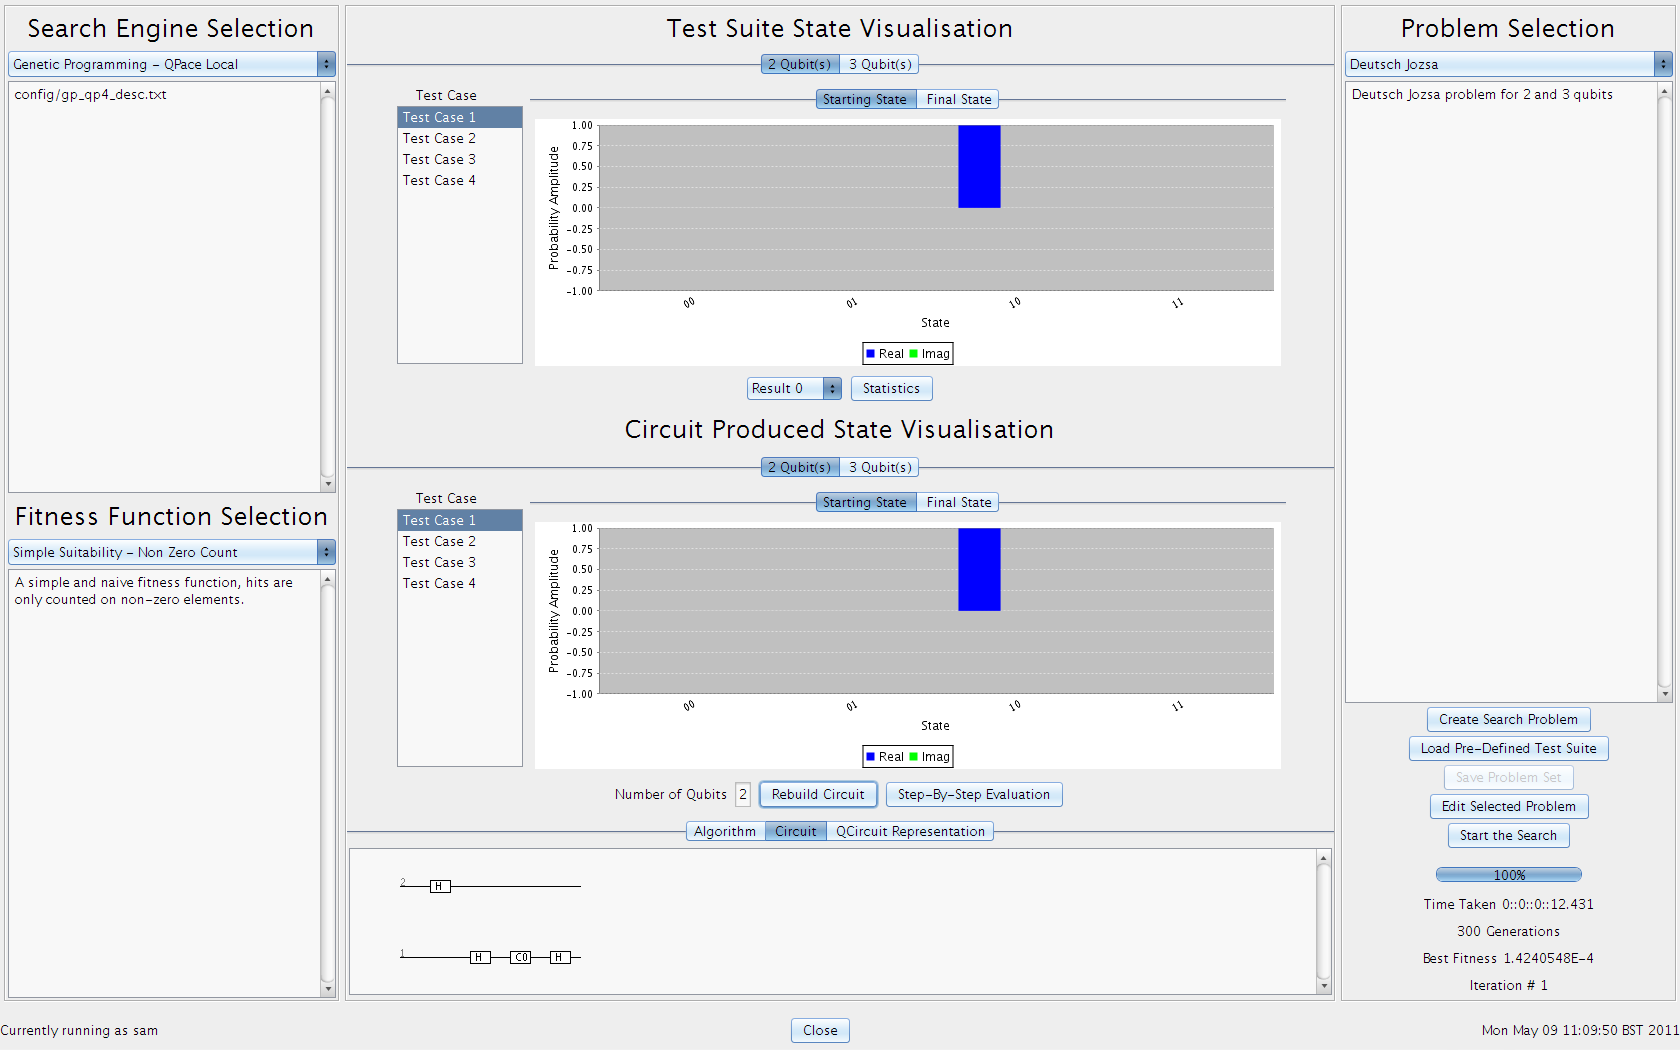
\includegraphics[width=\textwidth]{GUIDesign.png}
\caption{Main User Interface - After Search}
\label{fig:MainGUIDesign}
\end{figure}

Each section of the GUI is explained separately with reference to the principles listed.

\subsection{Main Window Layout}
As can be seen in Figure \ref{fig:MainGUIDesign} the layout of the main window separates the ``dissimilar things'' with the use of visible but subtle borders.
This meets the \emph{structure} principle.
The interface is structured so that the centre of the display contains the information of the highest importance, framed  by two control menus.
This central panel collates all of the main results of the latest search.
% The search statistics are shown in the right hand menu area.
% This separation ensures that the GUI does not become cluttered.

The layout is also intended to take into account the recent move towards wide screen monitors.
Wide screen monitors provide a new problem in GUI design.
If a GUI fills the screen area and fills it fully with the display of information, it can appear stretched and distorted.
If the GUI were to have a single menu along one side it also doesn't ``look right'', it looks excessively heavy on the non-menu side.
This is a issue with standard monitors also but in my opinion is exacerbated by the wide screen ratios.
Although it isn't directly related to any of the design principles it is an important property of a GUI to appear well balanced across the available screen area.

With the two menu panels the separation of the configuration options allows for a simple layout of configuration.
On the main window the only configuration that is available is the selection of the Search Engine, Suitability Measure and Search Problem.
The configuration of the Search Engine and the definition of the Search Problem is not handled by the main window.
This is to ensure that the display does not become overly cluttered, it maintains a simple and clean appearance.
This is a result of both the \emph{simplicity} and the \emph{visibility} principles.

\subsection{Search Engine, Suitability Measure and Search Problem Selection}
\label{sec:seselecdes}
\label{sec:smselecdes}
\label{sec:spselecdes}
Before a search can be started, selections have to be made for the Search Engine, Suitability Measure and Search Problem.
The selection of these are provided by three drop down lists.
The available options for a user to select are limited to the Search Engines and Suitability Measures that are registered in the respective managers in the framework.
For a user to add a new Search Engine or Suitability Measure the respective XML configuration file needs to be updated.
This was done so as to follow the \emph{simplicity} and \emph{tolerance} principles.
It ensures that any selection made by the user is a valid selection.

The selection of the Search Problem is again provided by a drop down list, following the \emph{simplicity} and \emph{tolerance} principles.
The difference is that the creation of a new problem from scratch and using a predefined test suite held in an XML file can be performed within the GUI.
Despite this difference, the use of the drop down list still ensures that any selection made by the user is a valid selection.
The validity of each individual Search Problem is checked by the editor dialogs described next.

All three of these selections are performed in the same way and ensure that the GUI maintains a level of consistency, meeting the \emph{reuse} principle.
When a selection is made, it is shown as selected and its description is displayed in the text area below, provided in the relevant configuration XML file, is shown.
The description areas are included to meet the \emph{feedback} principles and allow developers of Search Engines, Suitability Measures and indeed Search Problems to provide full text descriptions to the users from within the GUI.

\subsection{Search Problem Creator and Editor}
\label{sec:guisearchcreateed}
As mentioned above, the creation of Search Problems is provided by an on-screen dialog box.
The creation and editing of Search Problems is also provided by a standalone application, see Section \ref{sec:indtestsuiteeditor}.
The interface to includes an \emph{import from file} function.
This allows the user to register a new Search Problem using an XML file to define the test suite.
This allows researchers to easily register Search Problems created and distributed by other researchers.

The integrated editor and the standalone application use the same components and overall design.
The same components are also used when creating a new Search Problem and when editing an existing Search Problem.

Not only are the individual components reused but each dialog box follows the same design layout.
This promotes the \emph{reuse} and \emph{structure} principles.

The dialog boxes ensure that the user has entered values for the required fields and ensures that each entry is valid.
This implicitly ensures that each selection available to the user in the Search Problem drop down list is a valid option.
This follows the \emph{tolerance} principle.

\subsection{Reporting Results}
\label{sec:repres}

\begin{figure}
 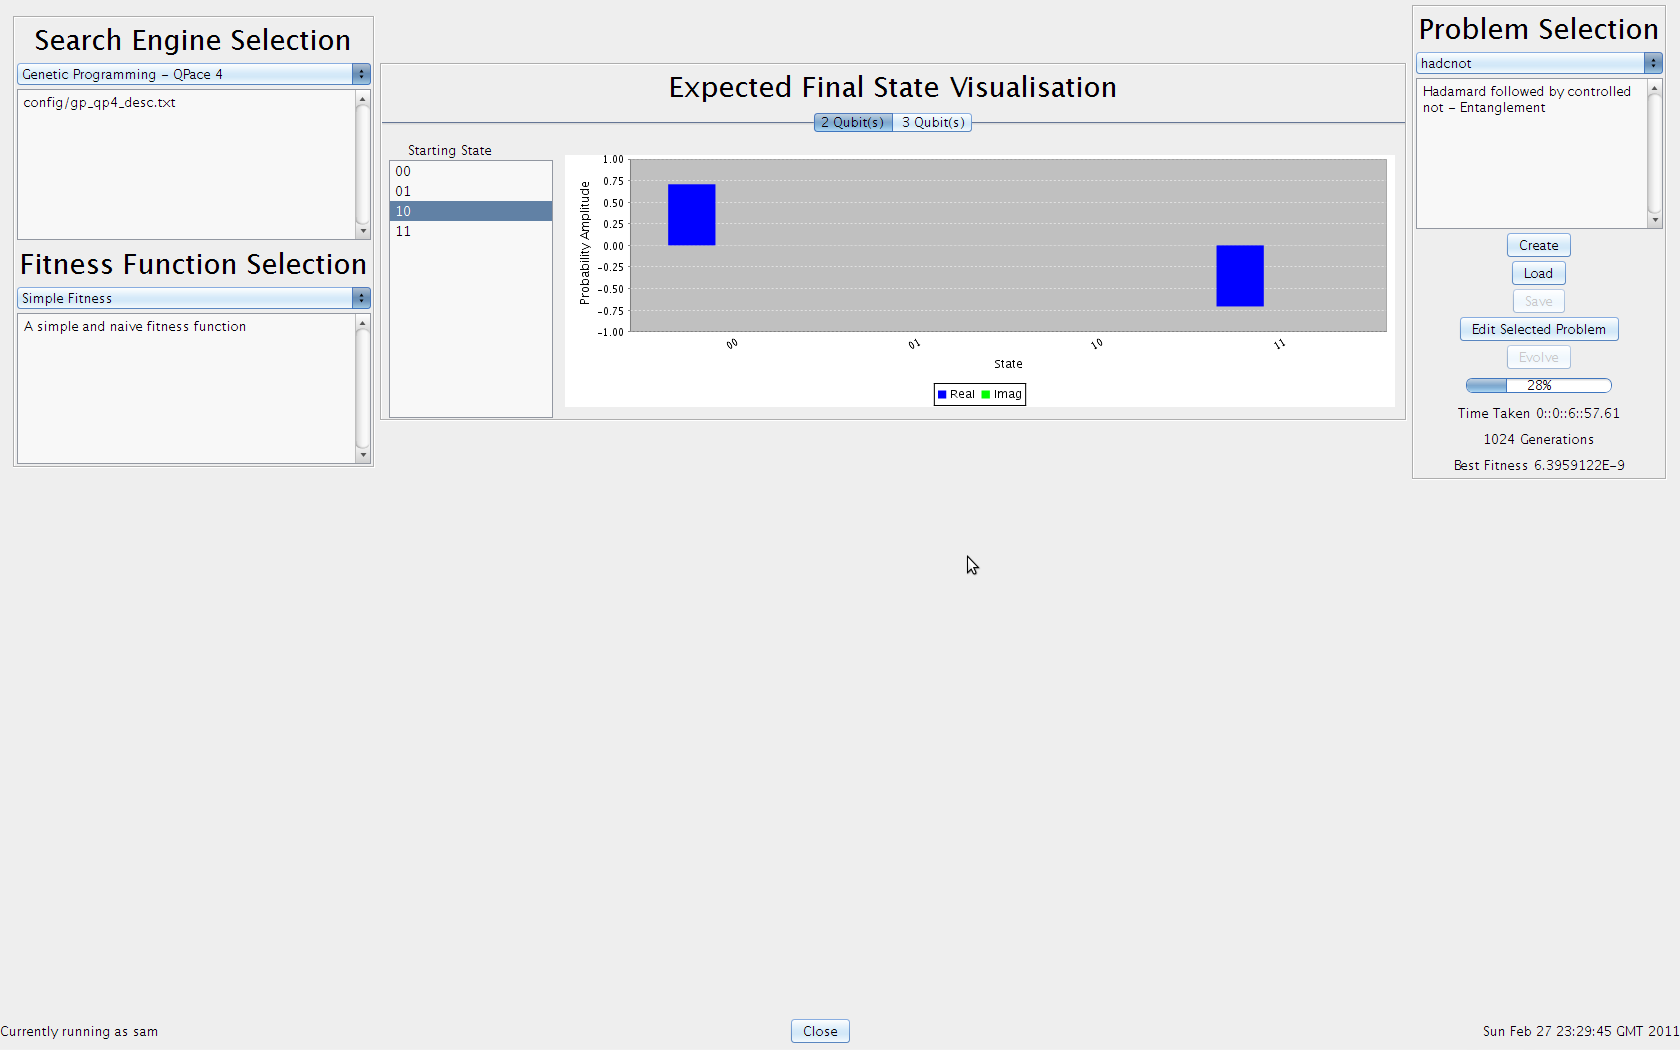
\includegraphics[width=\textwidth]{GUIDesignProgress.png}
\caption{Main User Interface - Before Search}
\label{fig:MainGUIDesignProg}
\end{figure}
\begin{figure}
 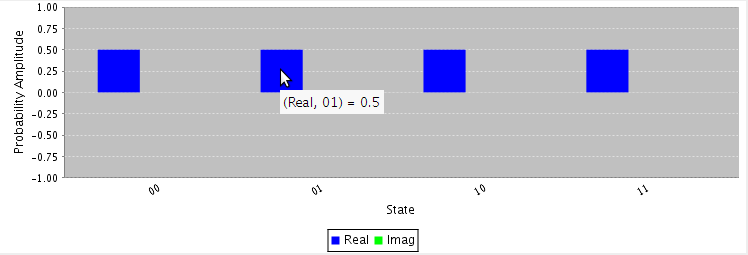
\includegraphics[width=\textwidth]{AccurateReadOutMouseOver.png}
\caption{Accurate State Readout}
\label{fig:AccStateReadOut}
\end{figure}
When a Search Problem is selected, in the central area a visual representation of the test suite is produced.
This representation can be seen in Figure \ref{fig:MainGUIDesignProg}.

After a search has been completed, the final states produced by the realised algorithm are shown using the same representation.
This can be seen in Figure \ref{fig:MainGUIDesign}.
Using a simple visualisation like this makes the comparison between ``desired'' final states and the final state produced by the algorithm found by the search.
It is true that the visualisation could be too simple for small differences to be noticed.
To counter this problem the visualisation allows the user to hover the mouse over each column to get an actual value.
This can be seen in Figure \ref{fig:AccStateReadOut}.

This provides users with both a quick, simple and visual way to compare final states as well as an accurate way to compare final states.
The accurate comparison method provided was implemented rather than a value table as part of following the \emph{simplicity} principle.

The result of a search is the quantum algorithm found by the search, rather than the final states for the test cases described so far.
The GUI provides the user 3 different ways to see the search result.
A simple textual listing of the algorithm is provided in the same format as the framework produces on its own.
To help with the users understanding of what the algorithm means a circuit diagram is produced for a user controlled number of Qubits.
The diagram is produced using the symbols that are shown in Figure \ref{fig:providedgates}.
The circuits produced are not just provided as a circuit diagram but also in QCircuit representation so that the circuits can be placed into any publication produced in Latex simply with the use of the QCircuit package.

Providing the three representations meet the \emph{simplicity}, \emph{feedback} and \emph{reuse} principles.
The \emph{simplicity} principle is met as the result of the search is simplified to a human readable algorithm and circuits can be created to help the user understand how the algorithm is working.
The \emph{feedback} principle is met as the circuit diagrams that are produced are done so using widely accepted symbols and conventions for quantum circuit drawing.
The \emph{reuse} principle is met with the use of QCircuit to produce circuits in a form that can be included in publications.
An alternative would have been to output the circuit diagram that is drawn by the GUI as an image that could have been included in any, not just Latex, publication.
I feel the use of QCircuit is a better choice as the user then has control and is able to carry out, if necessary, manual circuit optimisation.

\subsection{Step-By-Step Evaluator}
\label{sec:sbse}

\begin{figure}
 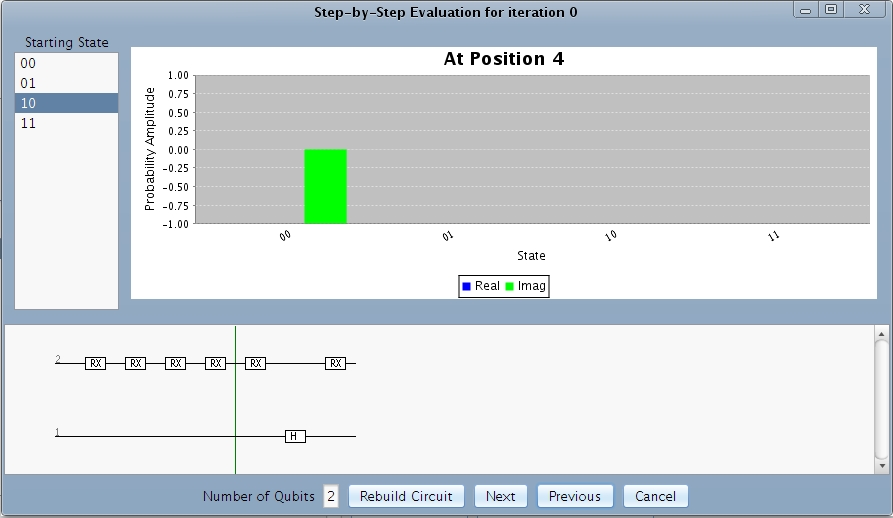
\includegraphics[width=\textwidth]{StepByStepEval.jpg}
\caption{Step-By-Step Evaluation Dialog}
\label{fig:StepByStepEval}
\end{figure}
The way in which quantum algorithms and the circuits they produce work is usually subtle and can be hard to understand by simply looking at the circuit.
The framework provides a step-by-step evaluation trace when provided with the input states.
The input states are provided to the framework in a test suite structure.
It was decided that the provided GUI would provide the test suite of the respective Search Problem.
This means that an evaluation trace is produced for each of the test cases, in each of the test suites.

The step-by-step evaluator is provided in a dialog box rather than integrated in the main frame.
This dialog box can be seen in Figure \ref{fig:StepByStepEval}.
This was done so as to focus the user's attention and to ensure that the addition of the functionality did not result in a cluttered GUI.
This follows the \emph{structure} and \emph{visibility} principles.

The step-by-step evaluation is performed with respect to a produced circuit.
This requires the user to select the number of qubits the circuit should be produced for and the step-by-step evaluation is provided for all test cases of that number of qubits.
Due to the design decision made for the framework, to provide a full trace rather than interactive evaluation, the test cases can be switched between at any step without returning to the start of the circuit.

The dialog box provides a circuit diagram, an initial state selector and a visual representation of the state at the ``current step'' in the evaluation for the selected initial state.
The circuit diagram is produced by reusing the circuit diagram drawn in the results pane of the main window.
This ensure that the circuit is represented using the same standards as that shown in the results pane.
The only difference is that the ``current step'' is indicated using a vertical line on the circuit diagram, this can be seen in Figure \ref{fig:StepByStepEval}.
This follows the \emph{reuse}, \emph{feedback},  \emph{visibility} and \emph{simplicity} principles.

The visual representation and initial state selector are the same as those used to report the final states produced for the test suite in the main window.
The only difference is that only the test cases for the current number of qubits is shown.
The use of the same visual representation ensure the user does not have to understand anything extra to use this functionality and follows the \emph{reuse} principle.

\section{Summary}

The design and implementation details outlined in the sections above cover all the functionality provided by the toolkit.




% \subsubsection{The Structure Principle}
% As can be seen in Figure \ref{fig:MainGUIDesign} the layout separates the ``dissimilar things'' with the use of headings and borders.
% The interface can be viewed as structued so that the centre of the display contains the information of the highest importance, straffed by two control menus.
% This central panel collates all of the result information regarding the result of the latest search.
% The search statistics are shown in the right hand menu area.
% This separation ensures that the GUI does not become cluttered.
% 
% This layout is also intended to take into account the recent move towards wide screen monitors.
% Wide screen monitors provide a new problem in GUI design.
% If a GUI fills the screen area and fills it fully with the display of information, it can appear stretched and distorted.
% If the GUI were to have a single menu along one side it also doesn't look ``right'', it looks excessively heavy on the non-menu side.
% This is a issue with standard monitors also but in my opinion is excasserbated by the wide screen ratios.
% 
% As well as the main GUI, the dialogs used to Create, Load and Edit search problems are all structured in such a way so as to guide a user through the respective operation.
% 
% The implemented search engine also provides a dialog box to configure a series of parameters.
% This dialog is split into two sections.
% One section contains a selection of all available gates while the second provides a series of GP parameters that the user may be interested in configuring, such as the number of generation and the population size.
% This separation follows the structure principle and clearly separates to the two distinct sets of configuration options.
% 
% \subsubsection{The Simplicity Principle}
% The way in which the framework has been designed aids in making the user interface simple.
% The framework requires very little configuration.
% The only real configuration that is required is the selection of which search engine and suitability measure to use and what problem you want to try solve.
% These selections are provided in very simple drop down lists for the users seletion.
% 
% The GUI provides a visual way to Create new and Edit existing search problems.
% A standalone editor is also provided.
% The editor provides a 
% 
% The only other two aspects of the configuration are the problem editor and the configuration of the search parameters.
% These are justified separately.
% 
% \subsubsection{The Visibility Principle}
% I think it is quite clear to see that the number of ``options'' visible to the user at any one time is minimised.
% The use of drop down boxes for selection naturally hides unwanted options until required.
% 
% In the central area the available selections are visible but are also much more likely to be ``browsed'' by the user.
% The decision not to use drop down boxes for the initial state selection is due to the expected ``browsing'' of this data.
% I expect that the user is likely to flick through the various options available which is much easier when the options are always visible.
% The use of a drop down box would also have required two mouse clicks per selection, one to open the list and one to make the selection.
% With the options visible this is reduced to a single click.
% 
% \subsubsection{The Feedback Principle}
% Once a selection is made for any of the selections available to the user the information on the display is updated accordingly.
% For example, the selection of a different search engine will update the contents of the search engine description area, selecting a different ``input state'' in the graph panels automatically updates the graph and the selection is highlighted.
% 
% 
% The user interface has been designed so that one user could leave it, a second user come to use it and understand very quickly the decisions that had already been made.
% It is not just the selection choices that are provided to the user as feedback.
% As can be seen in Figure \ref{fig:MainGUIDesignProg}, a progress bar is provided to indicate to the user how far through the current search the system is.
% 
% \subsubsection{The Tolerance Principle}
% To meet the tolerance principle the user interface has been designed to ensure that any user input is either restricted to valid inputs or validated on acceptance, notifying the user of any invalid input.
% A good example of this is the way the user selects the Search Engine, Suitability Measure and Search Problem.
% These selections use drop-down lists.
% This ensures that, assuming a correct implementation, any selection made by the user is valid.
% 
% For user input that is not limited to a small finite set of inputs, all user inputs are checked on and any incorrect input is brought to the users attention.
% This tolerance ensures that the system allows the user to correct any problems without loosing any other input.
% 
% As is noted in Section \ref{sec:introtoquantcomp} all quantum gates must be unitary.
% To ensure the system complies with this, when creating custom matricies for custom gates, the editor checks the matrix to ensure that it represents a unitary operation.
% 
% 
% 
% \subsubsection{The Reuse Principle}
% 
% Visualisation of similar information is shown using the same techniques.
% The use of tabs is two-fold.
% In the column chart panels it is used to select the data to show using the chart.
% In the lowest panel it is used to switch between the different representations of the solution that the system provides.
% 
% 
% \begin{itemize}
%  \item Extendible Library
% \end{itemize}